
\author{Markus Gronau}

\section{First steps}

  \subsection{Setting up the environment}
  For compiling and running java applets you need the Java Software Development Kit 
  (JDK/SDK) with the version 1.4.2 or newer.\\
  For viewing applets in your internet browser, you need a Java-plugin.\\
  Both can be obtained for free from \url{http://java.sun.com}.\\
  The Java APIDOC, the Java tutorial and the following extensions are also available there:
  \begin{itemize}
    \item Java3D for 3-dimensional graphics
    \item JavaMediaFramework (JMF) for screen capture support
  \end{itemize}
  
  You have to put the MathletFactory library (JAR-files) into the Java classpath
  where the compiler and the runtime will search for the classes (see your 
  Java documentation for information about setting the classpath).
  \\\\
  The use of a professional Integrated Development Editor (IDE) instead of a simple
  text editor is strongly encouraged. Here you can include the APIDOC and the sources
  into the editor for an easier programming.
  
  \subsection{Applet Skeleton Framework}

	With providing a flexible and powerful ``skeleton'' framework for applets, the developer has neither to
	``reinvent the wheel again'', nor to transfer whole passages of code for new programs. Instead, basing
	on an applet skeleton, mathlets have a generic interface for both the code itself and the placement of
	code. This simplifies the understanding of mathlet code (even if it is not the ``own'' code) and thus
	reduces developing and debugging time.

  \subsubsection{Structure of a mathlet}
  The class \codename{BaseApplet} is the base for all mathlets.
  It defines a common design where the components
  are placed into predefined panels/panes (containers able to hold GUI-components).
  The 3 main panels of a mathlet are (read from top to bottom):
  \begin{itemize}
    \item title pane containing a text panel with the mathlet's title
    \item center pane containing the canvases and/or a control-panel
    \item button pane containing the help, reset, screenshot and animation buttons
  \end{itemize}
  The center pane itself is divided into (from top to bottom)
  \begin{itemize}
    \item canvas pane containing a single canvas or an arrangement of several canvases
    \item controls pane pane containing a \cp
  \end{itemize}

  \subsubsection{The choice of a mathlet type}
  The mathlet-class needs to extend one of the template classes below.
  There are mathlet template types for the most common needs. The main distinction
  of theses templates is made by the number, the arrangement and the dimension of 
  their canvases. \\
  The following template types are available:
  \begin{itemize}
    \item {\bf"No-Canvas"} -- only 1 ControlPanel\\
      \[NoCanvasApplet\footnote{net.mumie.mathletfactory.appletskeleton}\]
    \item {\bf"Single"} -- 1 single canvas and 1 ControlPanel below\\
      \[2D: SingleG2DCanvasApplet\footnote{net.mumie.mathletfactory.appletskeleton.g2d}, 
      3D: SingleJ3DCanvasApplet\footnote{net.mumie.mathletfactory.appletskeleton.j3d}\]
    \item {\bf"Side-By-Side"} -- 2 canvases arranged horizontally and 1 ControlPanel below\\
      \[2D: SideBySideG2DCanvasApplet^{2}, 3D: SideBySideJ3DCanvasApplet^{3}\]
    \item {\bf"Upper-Lower"} -- 2 canvases arranged vertically and 1 ControlPanel below\\
      \[2D: UpperLowerG2DCanvasApplet^{2}\]
    \item {\bf"Upper-Middle-Lower"} -- 3 canvases arranged vertically and 1 ControlPanel below\\
      \[2D: UpperMiddleLowerG2DCanvasApplet^{2}\]
  \end{itemize}
  The ControlPanel resides below the canvases, except for the
  \verb|NoCanvasApplet|: there it covers the whole mathlet's space.
  
  \subsubsection{Creating the applet class}
  The "entry point" of every applet is the \verb|init()| method which will be called
  by the web-browser to load and initialize the applet.\\
  This is also true for a mathlet and its runtime: a call to the \verb|init()| method of the
  super class is necessary for initializing the system.\\
  An empty mathlet can look like this (e.g. for a "Single-Canvas"-applet):\\
  {\small\ttfamily
  \indent import net.mumie.mathletfactory.appletskeleton.g2d.*;\\\\
  \indent public class MyApplet extends SingleG2DCanvasApplet \{\\
  \indent \indent public void init() \{\\
  \indent \indent \indent super.init() // needed to initialize the runtime\\
  \indent \indent\indent ... // your entry point\\
  \indent \indent \}\\
  \indent \}\\
  }
  Note that the call \verb|super.init()| is needed to initialize the mathlet's runtime.
  
  \subsection{Basic User Interface}
  Every mathlet shares the same basic user interface with the following common features.
  
  \subsubsection{Title}
  The title is shown at top of the mathlet, i.e. above the canvases and the control panel.
  It can be set with\\
  \indent \verb|setTitle(String)|\\
  defined in the \verb|BaseApplet| class.
  
  \subsubsection{Reset Button}
  A generic reset button can be used to re-initialize a scene.\\
  The button itself can be added by simply calling \verb|addResetButton()| inside
  an extended BaseApplet-class. By pressing the button, the method 
  \verb|public void reset()| will be called in the mathlet. To react on this event
  you will have to overwrite this method in the applet-class.  
  
  \subsubsection{Dynamic Reset Button}
  
  \subsubsection{Screenshot Button}
  A generic screenshot button can be used to create screenshots and videos by capturing
  graphical scenes are the complete mathlet.\\
	The button will be visible when calling \verb|addScreenShotButton()| inside an
	extended BaseApplet-class.

  \subsubsection{Using Tabs}
    It is possible to open a new tab in the control-panel-, canvas- and center-pane.
    This is done by calling \verb|add(String, Component)| on the following getters:
    \begin{itemize}
      \item getCanvasTabbedPane()
      \item getCenterTabbedPane()
      \item getControlTabbedPane()
    \end{itemize}
  These methods return a customized instance of a JTabbedPane\footnote{javax.swing.JTabbedPane}
  (an instance of \verb|TabbedPanel| more precisly) which will show the real tab
  (with the tab's title) only when more than one tab has been added.\\
  Note: all of the BaseApplet's tabbed panes have allready a tab (containg the canvases, etc.).
  But the tab's titles are not visible because they are the only tabs!\\\\
  The add-method of these tabbed panes request a string for the tab's title and an
  instance of Component\footnote{java.awt.Component} which can be e.g. a new 
  ControlPanel, Canvas or JPanel (they all extends the class \verb|Component|).\\
  The title of the first (default) tab can be set through the \verb|TabbedPanel|-proper
  method \verb|setTitleAt(int, String)|.\\
  The instance of this underlying SWING-class
  can be accessed through \verb|getTabbedPane()| in the class \verb|TabbedPanel|.
  
  \subsection{Error Handling}
  Every action inside a mathlet can use the internal error handling system to provide a 
  \textit{quality feedback} of unexpected errors during the execution.\\
  In order to \textit{catch} an error, the following block must surround an action inside a mathlet:\\
  {\small\ttfamily
    \indent try \{\\
    \indent\indent ...\\
    \indent \} catch(Throwable t) \{\\
    \indent\indent reportError(t);\\
    \indent \}\\
  }
  The only actions during execution are the applet instance methods and actions inside the user interface
  (i.e. \textit{events}).
  
\newpage
\section{MM-Objects}
  \mmos (Multimedial Mathematical Objects) are the primary entities with which 
  an application programmer of the MathletFactory has to deal with. The MathletFactory 
  tutorial gives an overview of the framework that provides the simple use of \mmos. 
  This can be summarized in one sentence: \mmos encapsulate the mathematical and 
  interactivity state and are mapped onto graphic primitives (so called {\it drawables}) 
  and panel representation (so called {\it MMPanels}) by the use of specialised 
  {\it transformers}. The figure below shows the common role allocation in such a 
  \textit{Modell-View-Controller architecture}.
	\begin{figure}[h]
	  \begin{center}
	    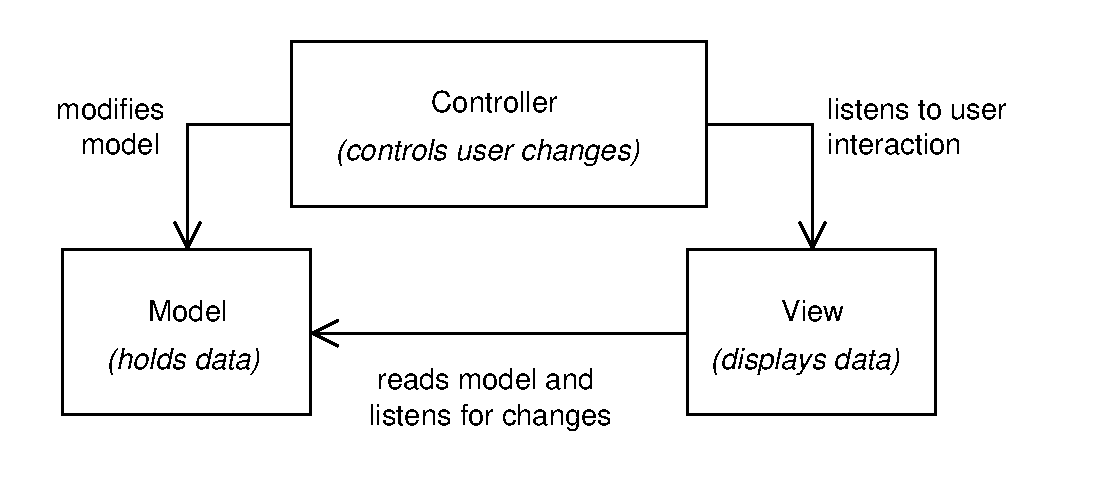
\includegraphics[width=10cm]
	      {images/mvc_common.pdf}
	    \caption{Common role allocation in a MVC architecture}
	    \label{fig:mvc_common}
	  \end{center}
	\end{figure}

  An \mmo is either a super class of a mathematical class\\(located in \verb|net.mumie.mathletfactory.math|)
  implementing the \verb|MMObjectIF| interface or an extension of the class \verb|MMDefaultCanvasObject|
  or \verb|DefaultMMObject|, implementing 
  itself this interface and its necessary methods.\\
  Note: \\
  \begin{itemize}
    \item -- every \mmo's name starts with the two capital letters "MM"
    \item -- every \mmo is located in the tree branch \verb|net.mumie.mathletfactory.mmobject|
  \end{itemize}
  
  
\subsection{Displaying MMObjects}
  A single \mmo can be displayed in multiple instances of container- and canvas drawables.
  (a "Container" means a box where GUI-elements such as buttons, labels and textfields
  can be added and displayed)(e.g. the \verb|ControlPanel| or a simple \verb|JPanel|).\\
  Thereby it is possible to display the \mmo's content for different transform types
  in separate drawables and even in multiple drawable instances for the same mathematical entity.
  
 \subsubsection{Representing content in Containers}
    Each time one of the methods
     \begin{itemize}
      \item getAsContainerContent()
      \item getAsContainerContent(int)
    \end{itemize}
    is called, a new container drawable instance will be created and returned. The first
    method returns the default container drawable, the second returns the drawable designated
    by the transform type. It is necessary to store it in a variable because these
    methods will never return this same instance again. The returned component can
    then by casted to the drawables runtime class to gain access to class specific 
    functionalities.
  
  \subsubsection{Representing content in Canvases}
    Each time one of the methods
     \begin{itemize}
      \item getAsCanvasContent()
      \item getAsCanvasContent(int)
    \end{itemize}
    is called, a new container drawable instance will be created and returned. The first
    method returns the default container drawable, the second returns the drawable designated
    by the transform type. It is necessary to store it in a variable because these
    methods will never return this same instance again. The returned component can
    then by casted to the drawables runtime class to gain access to class-specific 
    functionality.
    
  \subsection{Display Properties}
  Each \mmo has its own display properties which define appearance related settings such as colors,
  fonts or transparency. They can be returned and set with
  \begin{itemize}
    \item \verb|getDisplayProperties()|
    \item \verb|setDisplayProperties(DisplayProperties)|
  \end{itemize}
  Both methods are defined in the interface \verb|MMObjectIF|.\\
  Moreover some MM-classes have extended properties where special settings are
  possible. By casting to the \verb|DisplayProperties|-runtime class they offer additional methods to
  change other useful settings such as the line width, point radius or the basic shape of a drawable:\\
  \begin{footnotesize}
  \begin{verbatim}
  MMAffine2DPoint p1;
  // ... initializing the point ...
  PointDisplayProperties pdp = new PointDisplayProperties(p1.getDisplayProperties());
  pdp.setPointRadius(10);
  \end{verbatim}
  \end{footnotesize}
  Note that no copying of the properties of "p1" is actually done but a referencing of the internal property maps.
  It is possible to call \verb|clone()| on an instance of \verb|DisplayProperties| to copy the settings
  into a new independant instance:\\
  {\small\ttfamily
    DisplayProperties dp2 = (DisplayProperties) dp1.clone();\\
  }
  \\
  The following table shows the available DisplayProperties in \mmos and Drawables:\\\\
  {\small\ttfamily
  \begin{tabular}{|l|l|l|} \hline
    \rmfamily Properties-Class & \rmfamily implementing MM-Class & \rmfamily using Drawable\\ \hline\hline
    LineDisplayProperties & MMAffine2DLine & G2DLineDrawable\\
    & MMAffine2DLineSegment & J3DLineSegmentDrawable\\
    & MMAffine2DRay & J3DPolyLineDrawable\\
    & MMAffine3DLine & \\
    & MMAffine3DLineSegment & \\
    & MMCoordinateSystem & \\
    & MMDefaultRNVector & \\
    & MMVectorField2DOverR2- & \\
    & \indent\indent DefByComponents & \\
    & MMVectorField2DOverR2- & \\
    & \indent\indent DefByExpression & \\ \hline
    
    PointDisplayProperties & MMAffine2DPoint & G2DPointDrawable\\
    & MMAffine3DPoint & J3DPointDrawable\\
    & MMDefaultRN & \\
    & MMBezierPolynomialAdvanced & \\ \hline
    
    PolygonDisplayProperties & MMAffine2DPolygon & G2DPolygonDrawable\\
    & MMFunctionDefByOp & \\
    & MMFunctionDefinedByExpression & \\
    & MMFunctionDefinedBySamples & \\
    & MMPiecewiseFunction & \\
    & MMStepFunction & \\
    & MMBezierPolynomialAdvanced & \\
    & MMPolynomial & \\
    & MMParametricFunctionInR2 & \\
    & MMOneChainInR2 & \\ \hline
    
    SurfaceDisplayProperties & MMFunctionOverR2 & \rmfamily(no explicit drawable)\\
    & MMParametricFunctionInR3 & \\ 
    & MMAffine3DPlane & \\ 
    & MMAffine3DSubspace & \\ \hline
  \end{tabular}
  }
  
\subsection{Number class}
  Most \mmos (or maybe their underlying mathematical classes) are dependant of a number type,
  means calculations are made through the number-class-proper arithmetic operations/methods.\\
  All MM-classes need this number class as parameter for their constructors for initializing their
  internal fields with numbers of this class. A change of the class outside the constructor (i.e. after
  initializing) is generally not possible.\\
  The available number classes are (located in \verb|net.mumie.mathletfactory.math.number|):\\
  {\ttfamily
    MDouble, MComplex, MRational, MComplexRational, MBigRational, MInteger, MNatural, MRealNumber, Zmod5.\\
  }

  
\subsection{Rendering cycle}
  Each rendering cycle is started either by a canvas, by the mathlet author (calling a manual repaint on the \mmo with 
  the \verb|render()| method) or by a handler (calling itself the \verb|render()| method).\\
  The \mmo forwards the repaint request to all of its working transformers which will set the internal data
  of the \mmo's drawables accordingly to the actual mathematical content.\\
  Calling \verb|render()| on a \mmo is therefore equivalent to calling \verb|render()| on every transformer
  instance hold by the \mmo.\\
  \\
  \underline{Example: 2D point}\\
  The \verb|MMAffine2DTransformer| gets the coordinates of its "master" (here: \verb|Affine2DPoint|) and passes 
  them to its drawable (here: \verb|G2DPointDrawable|) which will draw a point at the new coordinates in the canvas.\\
  When dragging the point with the mouse, an instance of the class \verb|Affine2D|\-\verb|MouseTranslateHandler| will set 
  the new coordinates in the master (a \verb|MMAffine2DPoint|) and the rendering cycle will continue
  as described above.
  
  
\newpage
\section{Graphical Scenes with {\tt Canvas}}
  A canvas is a paint board where \mmos, images and text can be displayed. It can hold either 2- or 3-dimensional
  objects, their class is respectively \verb|MMG2DCanvas| or \verb|MMJ3DCanvas|, subclasses of \verb|MM2DCanvas| and
  \verb|MM3DCanvas|.\footnote{The distinction of two 2D and 3D canvas classes was made to allow in future releases
  the usage of other graphics implementations than the Java-proper ones (\textit{Graphics2D} and \textit{Java3D}).}
  The common class of these two different canvas types is \verb|MMCanvas|, where the biggest part of functionality
  is implemented.\\
  
\subsection{Common Functionalities}
  Objects can be added with\\
  \indent \verb|addObject(MMCanvasObjectIF|\footnote{net.mumie.mathletfactory.mmobject})\\
  defined in \verb|MMCanvas|\footnote{net.mumie.mathletfactory.display}.

\subsection{2D Canvas}

\subsection{3D Canvas}



\newpage
\section{User Interfaces with {\tt ControlPanel}}
  The \verb|ControlPanel|\footnote{net.mumie.mathletfactory.appletskeleton.util} 
  represents a container for GUI(Graphical User Interface)-components,
  providing a flexible text editor-like layout manager. It allows the programmer 
  to add components and to lay out them in the mathlet as easy as writing a text: the
  ControlPanel's height will be divided upon all lines where each of them can have
  a different horizontal alignment (left, right and center). Their height will be determined
  by the preferred sizes of their child components.\\\\
  The \cp is a base functionality of the BaseApplet and all of its
  extending classes. In most cases it is positioned under the canvases (except for
  the NoCanvasApplet: there it fills the whole vertical space). It can be accessed
  through \verb|BaseApplet.getControlPanel()| or used indirectly by one of the delegate
  methods defined in the BaseApplet. These delegaters are named after their
  implementations in the ControlPanel, except the \verb|add()| method: its corresponding
  delegate method is \verb|addControl()|.\footnote{This distinction was made
  to show the difference between the add-method defined in the Applet-class
  and this one.}\\
  It is possible to create a new ControlPanel-instance (e.g. in a standalone applet
  or in a new tab) but it is not necessary to do this in the predefined mathlet
  classes.
  
\subsection{Layout Mechanism}
  At the begin (means no object has been added yet) a "line pointer" starts at the first
  line and adds all following components to it. A line will be terminated by a line
  break. The pointer will then jump to the second line.\\
  Note that line alignments can only be done for the current row.\\
  It is possible to use tabstops and other space holders for a more exact positioning.
  
\subsection{Method Summary}
  \begin{itemize}
    \item \verb|add(JComponent)| -- adds a component to the actual line's end
    \item \verb|addText(String)| -- adds a {\tt TextPanel} with the given text
    \item \verb|addText(String, Color)| -- adds a {\tt TextPanel} with the given text and color
    \item \verb|addImage(String)| -- adds an image with the given file location
    \item \verb|insertLineBreak()| -- jumps to the next line
    \item \verb|insertLineBreak(int)| -- jumps \verb|int| lines downwards
    \item \verb|insertTab()| -- inserts a single tabstop
    \item \verb|insertTab(int)| -- inserts \verb|int| tabstops
    \item \verb|insertHSpace(int)| -- inserts a place holder with \verb|int| pixels width
    \item \verb|insertVSpace(int)| -- inserts a place holder with \verb|int| pixels height
    \item \verb|setLeftAlignment(), setCenterAlignment(), setRightAlignment()| -- sets left/center/right 
          alignment of the current and all following lines
    \item \verb|setScrollable(boolean)| -- sets whether the \cp should be scrollable
    \item \verb|getCurrentLine()| -- returns the container for the current line
    \item \verb|getLine(int n)| -- returns the container for the n-th line
  \end{itemize}



\newpage
\section{Styled Texts}

Styled texts can contain both descriptions, style and layout information.
They can be used in almost all applet technologies, except "raw" SWING components (e.g. \codename{JLabel}).

\subsection{Capable Components}

\subsubsection{\codename{TextPanel}}

  \underline{Package:} \codename{net.mumie.mathletfactory.display.util}\\
  This is the base component for all styled texts (i.e. TeX and HTML). 
  It is widely used in applets for e.g. titles and texts in \cps.
  It can be used as an replacement for \codename{JLabel}, which only supports HTML.\\
\\
Special methods:
  \begin{itemize}
    \item \textbf{\codename{setText(String)}} sets the text to be displayed
    \item \textbf{\codename{setWidth(int)}} sets the \textit{preferred width} of this text component; 
          setting this property will enable \textit{word wrapping}; \codename{-1} will restore the default size
    \item \textbf{\codename{setHeight(int)}} sets the \textit{preferred height} of this text component; 
          \codename{-1} will restore the default size
    \item \textbf{\codename{setHorizontalTextAlignment(int)}} sets the alignment along the x axis by using 
          one of the \codename{SwingConstants}
  \end{itemize}

\subsubsection{\codename{StyledTextButton}}

  \underline{Package:} \codename{net.mumie.mathletfactory.display.util}\\
  This component combines \codename{JButton}s along with the capability to display styled texts.



\subsection{Styled Texts Using TeX}

Descriptive texts with font styles and formulas can be easily created using a \textit{TeX dialect}.
It orientates on the common TeX commands and syntax but uses some simplifications and harmonisations.
It is designed to easily add new commands if they are needed. By now only the most used commands are
implemented.

\subsubsection{Special Considerations}

  \begin{itemize}
    \item \emph{Environments} must be defined in the following form:\\
          \codename{$\backslash$command\_name\{argument\_1\}\{argument\_2\}\{...\}}
    \item \emph{Packages} must not be declared
    \item \emph{Math Environment} (i.e. "\$") is not used
    \item \emph{Blanks and Line Breaks} are ignored
    \item \emph{Constants} are always expressed in uppercase letters \\(e.g. color constant "RED").
  \end{itemize}
  
\subsubsection{Using Special Characters}

  \begin{itemize}
    \item \textbf{Java} - the backslash character ("$\backslash$") must be double quoted, i.e. "$\backslash$$\backslash$"
    \item \textbf{MM-TeX} - the backslash character ("$\backslash$") must be expressed with "$\backslash$backslash\{\}"
    \item \textbf{Plain Text} (e.g. \textit{message files}, see ...) - no restrictions
  \end{itemize}

\subsubsection{Adding Space}

\paragraph{Line Breaks}
  \begin{itemize}
    \item $\backslash\backslash$ - adds a line break\\
  \end{itemize}

\paragraph{Blanks}
  \begin{itemize}
    \item $\backslash$\codename{quad} - adds a non-breaking space\\
    \item $\backslash$\codename{qquad} - adds a double non-breaking space
  \end{itemize}

\newpage
  
\subsubsection{Font Formattings}

\paragraph{Font Size}
  \begin{itemize}
    \item \codename{tiny, small, normalsize, large, Large, LARGE, huge}\\
          \underline{Example:} "\codename{$\backslash$large\{Text\}}" $\Rightarrow$ \large{Text} \normalsize{ }
  \end{itemize}

\paragraph{Font Style}
  \begin{itemize}
    \item $\backslash$\codename{textbf}\{\textit{...}\} - bold font\\
          \underline{Example:} "\codename{$\backslash$textbf\{Text\}}" $\Rightarrow$ \textbf{Text}
    \item $\backslash$\codename{textit}\{\textit{...}\} - italic font\\
          \underline{Example:} "\codename{$\backslash$textit\{Text\}}" $\Rightarrow$ \textit{Text}
  \end{itemize}

\paragraph{Superscripts}
  \begin{itemize}
    \item \codename{\^}\{\textit{...}\} - superscript\\
          \underline{Example:} "\codename{a\^{}2}" $\Rightarrow$ $a^2$
    \item \codename{\_}\{\textit{...}\} - subscript\\
          \underline{Example:} "\codename{a\_3}" $\Rightarrow$ $a_3$
    \item \codename{\_}\{\textit{...}\}\codename{\^}\{\textit{...}\} - both super- and subscript\\
          \underline{Example:} "\codename{a\^{}2\_3}" $\Rightarrow$ $a^2_3$
  \end{itemize}
\textbf{Note:} The paranthesises can be omitted if only a single character should be scripted.

\paragraph{Font Color}
  \begin{itemize}
    \item $\backslash$\codename{textcolor}\{\textit{color}\}\{\textit{...}\}\\
          with \textit{color} as a color constant (see below).\\
          \underline{Example:} "\codename{$\backslash$textcolor\{BLUE\}\{Text\}}" $\Rightarrow$ \textcolor{blue}{Text} \normalsize{ }
  \end{itemize}

The available colors constants are:\\
\codename{WHITE, BLACK\\
GRAY, LIGHT\_GRAY, DARK\_GRAY\\
RED, LIGHT\_RED, DARK\_RED\\
PINK, LIGHT\_PINK, DARK\_PINK\\
ORANGE, LIGHT\_ORANGE, DARK\_ORANGE\\
YELLOW, LIGHT\_YELLOW, DARK\_YELLOW\\
GREEN, LIGHT\_GREEN, DARK\_GREEN\\
MAGENTA, LIGHT\_MAGENTA, DARK\_MAGENTA\\
CYAN, LIGHT\_CYAN, DARK\_CYAN\\
BLUE, LIGHT\_BLUE, DARK\_BLUE
}


\subsubsection{Mathematical Environments}

  \begin{itemize}
    \item $\backslash$\codename{frac}\{\textit{nominator}\}\{\textit{denominator}\} - fractions\\
          \underline{Example:} "\codename{$\backslash$frac\{a\}\{b\}}" $\Rightarrow$ $\frac{a}{b}$ \normalsize{ }
    \item $\backslash$\codename{vec}\{\textit{...}\} - vector arrows\\
          \underline{Example:} "\codename{$\backslash$vec\{v\}}" $\Rightarrow \vec{v}$ \normalsize{ }
    \item $\backslash$\codename{norm}\{\textit{...}\} - vector norm\\
          \underline{Example:} "\codename{$\backslash$norm\{a\}}" $\Rightarrow ||a||$ \normalsize{ }
    \item $\backslash$\codename{det}\{\textit{...}\} - determinant border (matrices)\\
          \underline{Example:} "\codename{$\backslash$det\{a\}}" $\Rightarrow |a|$ \normalsize{ }
    \item $\backslash$\codename{abs}\{\textit{...}\} - absolute value\\
          \underline{Example:} "\codename{$\backslash$abs\{a\}}" $\Rightarrow |a|$ \normalsize{ }
    \item $\backslash$\codename{dot}\{\textit{...}\} - single dotted characters\\
          \underline{Example:} "\codename{$\backslash$dot\{a\}}" $\Rightarrow \dot{a}$ \normalsize{ }
    \item $\backslash$\codename{ddot}\{\textit{...}\} - double dotted characters\\
          \underline{Example:} "\codename{$\backslash$ddot\{a\}}" $\Rightarrow \ddot{a}$ \normalsize{ }
    \item $\backslash$\codename{bar}\{\textit{...}\} - horizontal top bar\\
          \underline{Example:} "\codename{$\backslash$bar\{a\}}" $\Rightarrow \bar{a}$ \normalsize{ }
    \item $\backslash$\codename{tilde}\{\textit{...}\} - tilde top bar\\
          \underline{Example:} "\codename{$\backslash$tilde\{a\}}" $\Rightarrow \tilde{a}$ \normalsize{ }
  \end{itemize}
  
  
\subsubsection{Special Characters and Umlaute}

\paragraph{Mathematical Operators}

\begin{center}
  \begin{tabular}{|c|l|} \hline
    \textbf{Glyph} & \textbf{Command}\\ \hline
    $\sim$ & $\backslash$sim\\ \hline
    $\simeq$ & $\backslash$simeq\\ \hline
    $\equiv$ & $\backslash$equiv\\ \hline
    $\approx$ & $\backslash$approx\\ \hline
    $\ne$ & $\backslash$ne\\ \hline
    $\cong$ & $\backslash$cong\\ \hline
    $\le$ & $\backslash$le\\ \hline
    $\ge$ & $\backslash$ge\\ \hline
    $\pm$ & $\backslash$pm\\ \hline
    $\mp$ & $\backslash$mp\\ \hline
    $\cdot$ & $\backslash$cdot\\ \hline
    $\nabla$ & $\backslash$nabla\\ \hline
    $\partial$ & $\backslash$partial\\ \hline
  \end{tabular}
  \begin{tabular}{|c|l|} \hline
    \textbf{Glyph} & \textbf{Command}\\ \hline
    $\forall$ & $\backslash$forall\\ \hline
    $\exists$ & $\backslash$exists\\ \hline
    $\in$ & $\backslash$in\\ \hline
    $\empty$ & $\backslash$empty\\ \hline
    $\infty$ & $\backslash$infty\\ \hline
    $\perp$ & $\backslash$perp\\ \hline
    $\rightarrow$ & $\backslash$rightarrow\\ \hline
    $\Rightarrow$ & $\backslash$Rightarrow\\ \hline
    $\leftarrow$ & $\backslash$leftarrow\\ \hline
    $\Leftarrow$ & $\backslash$Leftarrow\\ \hline
    $\leftrightarrow$ & $\backslash$leftrightarrow\\ \hline
    $\Leftrightarrow$ & $\backslash$Leftrightarrow\\ \hline
    $ $ & $ $\\ \hline
  \end{tabular}
\end{center}

\paragraph{Special Characters and Umlaute}

\begin{center}
  \begin{tabular}{|c|l|} \hline
    \textbf{Glyph} & \textbf{Command}\\ \hline
    \'{a} & $\backslash$'{}a\\ \hline
    \^{a} & $\backslash$\^{}a\\ \hline
    \`{a} & $\backslash$\`{}a\\ \hline
    \~{a} & $\backslash$\~{}a\\ \hline
    \"{a} & $\backslash$\"{}a\\ \hline
    \u{a} & $\backslash$ua\\ \hline
    \ae & $\backslash$ae\\ \hline
    \c{c} & $\backslash$cc\\ \hline
    \'{e} & $\backslash$'{}e\\ \hline
    \^{e} & $\backslash$\^{}e\\ \hline
    \`{e} & $\backslash$\`{}e\\ \hline
    \"{e} & $\backslash$\"{}e\\ \hline
    \'{i} & $\backslash$'{}i\\ \hline
    \^{i} & $\backslash$\^{}i\\ \hline
    \`{i} & $\backslash$\`{}i\\ \hline
    \"{i} & $\backslash$\"{}i\\ \hline
    \l & $\backslash$l\\ \hline
    \~{n} & $\backslash$\~{}n\\ \hline
    \'{o} & $\backslash$'{}o\\ \hline
    \^{o} & $\backslash$\^{}o\\ \hline
    \`{o} & $\backslash$\`{}o\\ \hline
    \~{o} & $\backslash$\~{}o\\ \hline
    \"{o} & $\backslash$\"{}o\\ \hline
    \o & $\backslash$o\\ \hline
    \oe & $\backslash$oe\\ \hline
    \ss & $\backslash$\"{}s, $\backslash$ss\\ \hline
    \'{u} & $\backslash$'{}u\\ \hline
    \^{u} & $\backslash$\^{}u\\ \hline
    \`{u} & $\backslash$\`{}u\\ \hline
    \"{u} & $\backslash$\"{}u\\ \hline
    \'{y} & $\backslash$'{}y\\ \hline
    \"{y} & $\backslash$\"{}y\\ \hline
    !` & !'\\ \hline
  \end{tabular}
  \begin{tabular}{|c|l|} \hline
    \textbf{Glyph} & \textbf{Command}\\ \hline
    \'{A} & $\backslash$'{}A\\ \hline
    \^{A} & $\backslash$\^{}A\\ \hline
    \`{A} & $\backslash$\`{}A\\ \hline
    \~{A} & $\backslash$\~{}A\\ \hline
    \"{A} & $\backslash$\"{}A\\ \hline
    \u{A} & $\backslash$uA\\ \hline
    \AE & $\backslash$AE\\ \hline
    \c{C} & $\backslash$cC\\ \hline
    \'{E} & $\backslash$'{}E\\ \hline
    \^{E} & $\backslash$\^{}E\\ \hline
    \`{E} & $\backslash$\`{}E\\ \hline
    \"{E} & $\backslash$\"{}E\\ \hline
    \'{I} & $\backslash$'{}I\\ \hline
    \^{I} & $\backslash$\^{}I\\ \hline
    \`{I} & $\backslash$\`{}I\\ \hline
    \"{I} & $\backslash$\"{}I\\ \hline
    \L & $\backslash$L\\ \hline
    \~{N} & $\backslash$\~{}N\\ \hline
    \'{O} & $\backslash$'{}O\\ \hline
    \^{O} & $\backslash$\^{}O\\ \hline
    \`{O} & $\backslash$\`{}O\\ \hline
    \~{O} & $\backslash$\~{}O\\ \hline
    \"{O} & $\backslash$\"{}O\\ \hline
    \O & $\backslash$O\\ \hline
    \OE & $\backslash$OE\\ \hline
    $ $ & $ $\\ \hline
    \'{U} & $\backslash$'{}U\\ \hline
    \^{U} & $\backslash$\^{}U\\ \hline
    \`{U} & $\backslash$\`{}U\\ \hline
    \"{U} & $\backslash$\"{}U\\ \hline
    \'{Y} & $\backslash$'{}Y\\ \hline
    \"{Y} & $\backslash$\"{}Y\\ \hline
    ?` & ?'\\ \hline
  \end{tabular}
\end{center}

\newpage

\paragraph{Greek Characters}

\begin{center}
  \begin{tabular}{|c|l|} \hline
    \textbf{Glyph} & \textbf{Command}\\ \hline
    $\alpha$ & $\backslash$alpha\\ \hline
    $\beta$ & $\backslash$beta\\ \hline
    $\gamma$ & $\backslash$gamma\\ \hline
    $\delta$ & $\backslash$delta\\ \hline
    $\epsilon$ & $\backslash$epsilon\\ \hline
    $\zeta$ & $\backslash$zeta\\ \hline
    $\eta$ & $\backslash$eta\\ \hline
    $\theta$ & $\backslash$theta\\ \hline
    $\iota$ & $\backslash$iota\\ \hline
    $\kappa$ & $\backslash$kappa\\ \hline
    $\lambda$ & $\backslash$lambda\\ \hline
    $\mu$ & $\backslash$mu\\ \hline
    $\nu$ & $\backslash$nu\\ \hline
    $\xi$ & $\backslash$xi\\ \hline
    $o$ & $\backslash$omicron\\ \hline
    $\pi$ & $\backslash$pi\\ \hline
    $\rho$ & $\backslash$rho\\ \hline
    $\sigma$ & $\backslash$sigma\\ \hline
    $\tau$ & $\backslash$tau\\ \hline
    $\upsilon$ & $\backslash$upsilon\\ \hline
    $\phi$ & $\backslash$phi\\ \hline
    $\chi$ & $\backslash$chi\\ \hline
    $\psi$ & $\backslash$psi\\ \hline
    $\omega$ & $\backslash$omega\\ \hline
  \end{tabular}
  \begin{tabular}{|c|l|} \hline
    \textbf{Glyph} & \textbf{Command}\\ \hline
    $A$ & $\backslash$Alpha\\ \hline
    $B$ & $\backslash$Beta\\ \hline
    $\Gamma$ & $\backslash$Gamma\\ \hline
    $\Delta$ & $\backslash$Delta\\ \hline
    $E$ & $\backslash$Epsilon\\ \hline
    $Z$ & $\backslash$Zeta\\ \hline
    $H$ & $\backslash$Eta\\ \hline
    $\Theta$ & $\backslash$Theta\\ \hline
    $I$ & $\backslash$Iota\\ \hline
    $K$ & $\backslash$Kappa\\ \hline
    $\Lambda$ & $\backslash$Lambda\\ \hline
    $M$ & $\backslash$Mu\\ \hline
    $N$ & $\backslash$Nu\\ \hline
    $\Xi$ & $\backslash$Xi\\ \hline
    $O$ & $\backslash$Omicron\\ \hline
    $\Pi$ & $\backslash$Pi\\ \hline
    $R$ & $\backslash$Rho\\ \hline
    $\Sigma$ & $\backslash$Sigma\\ \hline
    $T$ & $\backslash$tau\\ \hline
    $Y$ & $\backslash$Upsilon\\ \hline
    $\Phi$ & $\backslash$Phi\\ \hline
    $X$ & $\backslash$Chi\\ \hline
    $\Psi$ & $\backslash$Psi\\ \hline
    $\Omega$ & $\backslash$Omega\\ \hline
  \end{tabular}
\end{center}


\subsection{Styled Texts Using HTML}


\newpage
\section{Internationalization}
  Internationalization of mathlets can be done by using localizable messages (identified
  by keys) for e.g. the title or descriptions inside the mathlet.
  The mathlet developer is encouraged to use localizable messages instead of static
  strings in order to free the code from language dependant expressions
  and therefore to provide a more flexible language integration.\\\\
  At start-up, the mathlet tries to load the correct message set for the executing system,
  else it tries to load it in the default language (english).
  
  \subsection{About Locales}
  In order to load the correct message set, the \textit{locale} of the executing system must 
  correspond to that of the message set.
  Each language has its own locale, e.g. "en" for english, "de" for german or
  "fr" for french. This language prefix identifies a set of messages/texts.\\
  The locale of the mathlet runtime can be set via properties/parameters, otherwise the system
  locale will be used.
  
  \subsection{Storing messages}
  
  There are two possibilities to store messages outside a mathlet, whereas it is possible to combine them.

  \subsubsection{Messages Files}
  Message files confirm to the Java Property Format and store the messages of a single set
  (i.e. for a single language) in an own file. The syntax is \codename{key = message}.
  The filename of a message-file is determined by the prefix
 "{\tt Messages\_"} followed by the locale and the file ending "{\tt .properties}"
  (e.g. {\tt Messages\_en.properties} for english). This file must reside in the mathlet's \textit{files directory}.\\
  A message in the "en" set could be:\\
  \indent myApplet.title = This is the title in english!\\
  whereas in the "de" set:\\
  \indent myApplet.title = Dies ist der Titel auf deutsch!\\
  
  \subsubsection{Messages Properties}
  Sets of messages can also be defined via XML in a mathlet's property file.\\
  Inside a "i18n" section a single message is defined by three attributes: the key, the language and
  the text/message.\\
  A {\tt messages} (plural!) section defines a set or sub-set of messages with at least one common
  attribute. By this way sets of messages can be organized e.g. by the language or the title in a 
  hierarchical structure.\\
  The "leaf" nodes must be concretemessages defined each in a {\tt message} (singular!) node.\\
  The following examples define three identical sets of messages:\\
  \underline{Example 1:}\\
  {\small\ttfamily
    \indent <mf:i18n>\\
    \indent\indent <mf:message key="title" language="en" value="Example Title"/>\\
    \indent\indent <mf:message key="title" language="de" value="Beispiel-Titel"/>\\
    \indent </mf:i18n>\\
  }
  \underline{Example 2:}\\
  {\small\ttfamily
    \indent <mf:i18n>\\
    \indent\indent <mf:messages key="title">\\
    \indent\indent\indent <mf:message language="en" value="Example Title"/>\\
    \indent\indent\indent <mf:message language="de" value="Beispiel-Titel"/>\\
    \indent\indent </mf:messages>\\
    \indent </mf:i18n>\\
  }
  \underline{Example 3:}\\
  {\small\ttfamily
    \indent <mf:i18n>\\
    \indent\indent <mf:messages language="en">\\
    \indent\indent\indent <mf:message key="title" value="Example Title"/>\\
    \indent\indent </mf:messages>\\
    \indent\indent <mf:messages language="de">\\
    \indent\indent\indent <mf:message key="title" value="Beispiel-Titel"/>\\
    \indent\indent </mf:messages>\\
    \indent </mf:i18n>
  }
  
  \subsubsection{Messages File Definitions}
  Inside a "i18n" section it is possible to include additional messages from custom messages files.
  In the following example, a messages file for each language will be defined:\\
  \underline{Example:}\\
  {\small\ttfamily
    \indent <mf:i18n>\\
    \indent\indent <mf:message-file language="de" file="my\_messages\_de.properties"/>\\
    \indent\indent <mf:message-file language="en" file="language\_en.ini"/>\\
    \indent </mf:i18n>\\
  }
  Note that the filenames here must not confirm to the common filename convention mentioned above.\\
  If a defined file is not found during the runtime start, an exception will be thrown. This can be
  omitted with the additional attribute \codename{mustExist} with the value \codename{false}.
  By this way, naming conventions for additional messages files can be declared (as for the common
  filename convention).\\
  \underline{Example:}\\
  {\small\ttfamily
    \indent <mf:i18n>\\
    \indent\indent <mf:message-file language="en" file="Messages\_en.properties"\\
    \indent\indent\indent mustExist="false"/>\\
    \indent </mf:i18n>\\
  }
  
  \subsection{Parametrised Messages}
  Sometimes a message does not only contain a static text but may also include \textit{variable content}.
  Instead of splitting the text around this content, placeholders can be used inside the text definition.
  The values they represent are defined in a list which must be specified while retrieving the message.
  Their name corresponds to the respective \textit{position} of their value in the list, prefixed with
  a "\$" character. The numbering starts as usual at "1". It is possible to use the same placeholder 
  multiple times in a message.\\
  If the list does not contain the appropriate number of items, an exception will be thrown.\\\\
  The following example demonstrates a message with two variables:\\
  \underline{Example:}\\
  {\small\ttfamily
    \indent my\_text\_key = The value is \$1 but must be \$2.\\
  }\\
  This message must be retrieved with a list of two values. The list could be created as follows:\\
  \underline{Example:}\\
  {\small\ttfamily
    \indent Object[] list = new Object[] \{ "my value 1", "my value 2" \};\\
  }
  See the next section for more information about retrieving messages.
  
  \subsection{Retrieving Messages}
  Messages of the current set can be retrieved through the two {\tt getMessage(...)} 
  methods defined in the {\tt BaseApplet}-class.\\\\
  The first method only takes a {\tt String} argument which represents the key:\\
  {\small\ttfamily
    \indent public String getMessage(String key)
  }\\
  Note that only non-parametrised messages can be retrieved with it.\\\\
  The second method has an additional argument for the list of parameters:\\
  {\small\ttfamily
    \indent public String getMessage(String key, Object[] params)
  }\\
  It allows to retrieve parametrised messages with the given parameters.\\\\
  \underline{Examples:}\\
  {\small\ttfamily
    \indent setTitle(getMessage("title"));\\
    \indent setTitle(getMessage("my\_text\_key",\\
    \indent\indent\indent new Object[] \{ "my value 1", "my value 2" \}));\\
  }\\
  Both methods return \codename{null} if no message is found in the current set.

\newpage
\section{Deploying Mathlets}
  There are some different possibilities to deploy own mathlets. Common to all of them is that
  the \mf library must be deployed with.

  \subsection{Applets}
  The browser plugin (or the \textit{appletviewer}) needs a website (i.e. a HTML or XHTML page)
  with proper "applet" or "object" tag to start the applet. This tag must include
  the location of the compiled classes, the applet size inside the page and may define
  other Plug-In settings and user-specified parameters.

  \subsubsection{Applet Tag}
  Applets may be embedded in websites with an \verb|<applet>| tag.\\
  Note that this tag is deprecated by the W3C in favor of the \verb|<object>| tag (see next section)
  but is also preferred by some browser plugins.\\
  The following example shows the usage of the \verb|<applet>| tag:
  \begin{verbatim}
    <applet code="MyApplet.class" codebase="." 
            archive="MyApplet.jar" width="400" height="300">
      <param name="myParameter1" value="a value">
      <param name="myParameter2" value="a value">
    </applet>
  \end{verbatim}
  \underline{Attributes:}
  \begin{itemize}
  \item \verb|code| specifies the name of the applet with or without suffix ".class". Note that no path must be specified!
  \item \verb|codebase| specifies the path to the class-file relative to the website's location
  \item \verb|archive| specifies a comma-separated list of needed archive files (i.e. "jar" or "zip" 
        files where also the applet class can be located in)
  \end{itemize}
  
  \subsubsection{Object Tag}
  Applets may also be embedded in websites with an \verb|<object>| tag.\\
  The usage of this tag is encouraged by the W3C.
  Below is an example for an \verb|<object>|-tag:
  \begin{verbatim}
    <object classid="java:MyApplet.class" codetyte="application/java"
          codebase="./" archive="MyApplet.jar" width="400" height="300">
      <param name="myParameter1" value="a value">
      <param name="myParameter2" value="a value">
    </object>
  \end{verbatim}
  \underline{Attributes:}
  \begin{itemize}
  \item \verb|classid| specifies the name of the applet with prefix "java:" and suffix ".class". Note that no path must be specified!
  \item \verb|codebase| specifies the path to the class-file relative to the website's location
  \item \verb|archive| specifies a comma-separated list of needed archive files (i.e. "jar" or "zip" 
        files where also the applet class can be located in)
  \end{itemize}

  \subsection{Applications}
  Applications runs in an own virtual machine outside the browser (e.g. from the command line).
  Hence some functionality must be added to satisfy the specific applet requirements.
  Starting an applet as an application means basically to perform these steps:
  \begin{itemize}
  \item create a {\tt main} method; this is the entry point for applications; the applet class
        must be created and initialized here
  \item call the applet instance methods {\tt init} and {\tt start} in order to initialize the 
        applet correctly
  \item create a frame where the applet should be put into and show that frame
  \end{itemize}
  
  These steps can be summarised as in the following example:\\
  {\small\ttfamily
  \indent import net.mumie.mathletfactory.appletskeleton.g2d.*;\\\\
  \indent import net.mumie.mathletfactory.util.*;\\\\
  \indent public class MyApplet extends SingleG2DCanvasApplet \{\\
  \indent\indent int width = 400, height = 300;\\
  \indent\indent public static void main(String[] args) \{\\
  \indent\indent\indent MyApplet applet = new MyApplet();\\
  \indent\indent\indent applet.init();\\
  \indent\indent\indent applet.start();\\
  \indent\indent\indent BasicApplicationFrame frame = \\
  \indent\indent\indent\indent\indent\indent new BasicApplicationFrame(applet, width, height);\\
  \indent\indent\indent frame.show();\\
  \indent\indent\}\\
  \indent\}\\
  }


\begin{appendix}

%\chapter{Miscellaneous Topics}

\end{appendix}